\pdfoutput=1
\documentclass[11pt]{amsart}

\usepackage[margin=1in]{geometry}
\usepackage{amsmath,amssymb,amsthm}
\usepackage{booktabs,longtable,array}
\usepackage{tikz}
\usepackage[hidelinks]{hyperref}

\newcommand{\NCand}{70}
\newcommand{\NRefl}{27}
\newcommand{\NNon}{44}
\newcommand{\NCerts}{167}
\newcommand{\NNew}{6}
\newcommand{\NEntries}{522}


\newtheorem{theorem}{Theorem}[section]
\newtheorem{lemma}[theorem]{Lemma}
\newtheorem{proposition}[theorem]{Proposition}
\newtheorem{corollary}[theorem]{Corollary}
\newtheorem*{hypothesis}{Hypothesis~(D)}
\theoremstyle{definition}
\newtheorem{definition}[theorem]{Definition}
\newtheorem{remark}[theorem]{Remark}

\newcommand{\Z}{\mathbb{Z}}
\newcommand{\Q}{\mathbb{Q}}
\newcommand{\R}{\mathbb{R}}
\newcommand{\Hy}{\mathbb{H}}
\newcommand{\OK}{\mathcal{O}}
\newcommand{\eps}{\varepsilon}
\newcommand{\id}{\mathrm{id}}
\newcommand{\N}{\mathrm{N}}
\newcommand{\Nmax}{\mathcal{N}}
\newcommand{\lab}[1]{\texttt{#1}}

\title[{Reflectivity of $-dx_0^2+x_1^2+\dots+x_n^2$ over $\Z[\sqrt2]$}]{Reflectivity of the quadratic forms
$-d\,x_0^2+x_1^2+\dots+x_n^2$ over $\Z[\sqrt2]$:\\ a computer-assisted classification}
\author{John Mcleod}
\date{\today}

\begin{document}

\begin{abstract}
Let $\OK=\Z[\sqrt2]$ and let $d\in\OK$ be squarefree with $d>0>\sigma(d)$, where $\sigma$ is
the non-trivial Galois automorphism. The form $f_d^n=-d\,x_0^2+x_1^2+\dots+x_n^2$ then defines a
cocompact arithmetic group $O'(f_d^n,\OK)$ acting on $\Hy^n$. We study for which $(d,n)$ this
group is generated by reflections up to finite index. A monotonicity lemma shows that the
reflective $n$ for a fixed $d$ form an interval $\{2,\dots,\Nmax(d)\}$. In particular,
$f_d^n$ reflective for some $n$ forces $\langle -d,1,1\rangle$ to be reflective, so it should
appear in A.~Mark's classification of strongly squarefree reflective rank-3 lattices over
$\OK$. Mark's table yields \NCand{} candidate values of~$d$. For each of them, and for one
further value, we determine $\Nmax(d)$ by our own Vinberg runs together with exactly
checkable certificates of non-reflectivity at $\Nmax(d)+1$. There are \NRefl{} reflective $d$,
with $\Nmax(d)\in\{2,\dots,6\}$, and \NNon{} values that are non-reflective in every dimension.
Six reflective pairs $(d,n)$ appear to be new, including new compact Coxeter polytopes in
dimensions 3, 4 and 5. One of them is $d=-1+3\sqrt2$, $n=2$: the lattice
$\langle 1-3\sqrt2,1,1\rangle$ is reflective with a compact hexagonal chamber, but it is
isometric to no entry of Mark's table, so that table is incomplete. Completeness of our list
therefore rests on an explicit, weaker hypothesis about the determinants occurring in Mark's
table, which we state and discuss. All decisions use exact arithmetic in $\Q(\sqrt2)$, and
all certificates are re-checkable by an independent verifier.
\end{abstract}
\maketitle

\section{Introduction}

Let $K=\Q(\sqrt2)$ with ring of integers $\OK=\Z[\sqrt2]$ and embeddings
$\id\colon\sqrt2\mapsto\sqrt2$ and $\sigma\colon\sqrt2\mapsto-\sqrt2$. We write
$\N(x)=x\,\sigma(x)$ and $\eps=1+\sqrt2$; then $\OK^\times=\pm\eps^{\Z}$ and $\N(\eps)=-1$.
Call $d\in\OK$ \emph{admissible} if $d>0$ and $\sigma(d)<0$. For admissible $d$ and $n\ge2$ the
form
\[
  f_d^n = -d\,x_0^2+x_1^2+\dots+x_n^2
\]
has signature $(n,1)$ at $\id$ and is positive definite at $\sigma$. So
$\Gamma_d^n=O'(f_d^n,\OK)$ is a cocompact arithmetic lattice in $\mathrm{Isom}(\Hy^n)$
\cite{Vin72,Bel16}. The lattice $L_d^n=\OK^{n+1}$ with this form is \emph{reflective} if the
subgroup $W_d^n$ generated by reflections in roots has finite index in $\Gamma_d^n$. This is the
cocompact analogue of the families $-p\,x_0^2+x_1^2+\dots+x_n^2$ over $\Z$ studied
in~\cite{Mc11,McTh,Mar15}. The classical example in our family is $d=\eps$, which is
reflective if and only if $n\le6$~\cite{Bug90}.

\subsection*{Results}
We call $d$ \emph{squarefree} if the ideal $(d)$ is.
\begin{enumerate}
\item \textbf{Monotonicity} (Lemma~\ref{lem:mono}). If $f_d^{n+1}$ is reflective, so is $f_d^n$.
  Hence the reflective $n$ for each $d$ form an interval $\{2,\dots,\Nmax(d)\}$, which may be
  empty.
\item \textbf{Reduction to Mark's table} (\S\ref{sec:reduction}). If $f_d^n$ is reflective for
  some $n$, then $\langle -d,1,1\rangle$ is a reflective strongly squarefree rank-3 lattice. By
  Mark's theorem~\cite{Mar18} it is then isometric to an entry of her table, so $(d)$ is the
  determinant ideal of an entry. The \NEntries{} entries of the table give \NCand{} distinct
  ideals, hence \NCand{} candidate values of $d$.
\item \textbf{Unconditional results} (Theorem~\ref{thm:main}). For each of the \NCand{}
  candidates and one further value, $\Nmax(d)$ is determined exactly
  (Table~\ref{tab:reflective} and Appendix~\ref{app:candidates}):
  \NRefl{} values have $\Nmax(d)\ge2$ and \NNon{} have $\Nmax(d)<2$. Every claim is backed
  either by a terminating Vinberg run, cross-checked with CoxIter, or by a certificate of
  non-reflectivity checked in exact arithmetic.
\item \textbf{A gap in Mark's table} (\S\ref{sec:gap}). The lattice
  $\langle 1-3\sqrt2,1,1\rangle$ ($d=-1+3\sqrt2$, a prime above $17$) is reflective with
  chamber a compact hexagon of angles $(\pi/8,\pi/4,\pi/2)^2$. It is isometric to none of
  the table entries.
\item \textbf{Completeness, conditionally} (Theorem~\ref{thm:conditional}). Assume
  Hypothesis~(D): every reflective strongly squarefree rank-3 lattice over $\OK$ has the
  determinant ideal of some table entry. Then Table~\ref{tab:reflective} lists every
  squarefree admissible $d$ for which $f_d^n$ is reflective for some $n$. Mark's theorem as
  stated would imply (D), but it fails at the level of individual lattices. The p17a
  counterexample does not contradict (D) itself, because its determinant ideal does occur
  in the table.
\item \textbf{New cases} (\S\ref{sec:literature}). Six reflective pairs $(d,n)$ are not in the
  sources we checked~\cite{Bug90,Mar18,Bog20,Gug17}. They are $(-1+3\sqrt2,2)$, $(\sqrt2,4)$,
  $(\sqrt2,5)$, $(1+2\sqrt2,4)$, $(3+3\sqrt2,3)$ and $(-2+3\sqrt2,3)$. For all $d$ except
  $\eps$ and $-1+2\sqrt2$, the upper end $\Nmax(d)$ appears to be new.
\end{enumerate}

\subsection*{Organisation}
\S\ref{sec:setup} fixes notation and conventions. \S\ref{sec:mono} proves the monotonicity
lemma. \S\ref{sec:reduction} gives the reduction from Mark's table to the list of candidates,
including how the table was extracted and checked. \S\ref{sec:vinberg} describes our
implementation of Vinberg's algorithm and \S\ref{sec:certificates} the certificates of
non-reflectivity. \S\ref{sec:results} states the results, \S\ref{sec:gap} discusses the gap
in Mark's table and the hypothesis on which completeness rests, and \S\ref{sec:literature}
compares with the literature. \S\ref{sec:calibration} lists the calibrations and
cross-checks, and \S\ref{sec:repro} explains how to reproduce everything.

\section{Setup and conventions}\label{sec:setup}

\subsection{Arithmetic in $\OK$}
Elements of $K$ are represented exactly as $a+b\sqrt2$ with $a,b\in\Q$. The sign of
$a+b\sqrt2$ is decided exactly: it is the common sign of $a$ and $b$ if they agree, and
otherwise it is decided by comparing $a^2$ with $2b^2$. Every positivity test in this work
(inequalities at $\id$, at $\sigma$ or at both) goes through this function. Floating-point
numbers are used only to order batches of candidates and inside one lattice-point
enumeration (\S\ref{sec:vinberg3}), where every output is re-checked exactly; they never
accept or reject anything. $\OK$ is norm-Euclidean, which gives gcds and factorisation.

\subsection{Canonical parameters}\label{sec:canonical}
A unit $u=\pm\eps^k$ is totally positive if and only if $u=\eps^{2j}$, i.e.\ iff it is a unit
square. Multiplying a generator of an ideal by a suitable unit $\pm\eps^k$ gives any sign
pattern, because $\eps$ has signs $(+,-)$. So the admissible generators of a given ideal form
a single orbit $d\,\eps^{2\Z}$. Moreover $x_0\mapsto\eps^k x_0$ shows that $f_d^n$ and
$f_{d\eps^{2k}}^n$ are isometric. Hence \emph{admissible squarefree $d$ up to isometry of
$f_d^n$ correspond bijectively to squarefree ideals $\mathfrak a\ne0$ of $\OK$}. For each
ideal we fix the canonical generator $\mathrm{can}(\mathfrak a)$ that minimises
$\max(|d|,|\sigma d|)$; ties are broken by the larger value at $\id$. Throughout, $d$ denotes
this canonical generator, and parameters carry short labels: \lab{unit} ($\eps$), \lab{ram2}
($\sqrt2$), \lab{inert3} ($3\eps$), \lab{p7a}/\lab{p7b} (the two primes above 7), and
\lab{dA\_B} or \lab{dmA\_B} for $\pm A+B\sqrt2$.

For a split rational prime $p=\mathfrak p\mathfrak p'$ the two primes are genuinely different
parameters: if $\pi$ is admissible so is $-\sigma(\pi)$, which generates $\mathfrak p'$, but
$f_\pi$ and $f_{-\sigma\pi}$ are not related by Galois conjugation with respect to the fixed
time-like embedding $\id$. The partner $d\mapsto -\sigma(d)$ plays a role in \S\ref{sec:gap}.

\subsection{Roots and reflectivity}
A \emph{root} of an $\OK$-lattice $L$ is a primitive vector $e\in L$ with totally positive
norm $m=(e,e)$ such that $2(e,x)/m\in\OK$ for all $x\in L$. The reflection
$r_e(x)=x-2\frac{(e,x)}{m}e$ then preserves $L$. Rescaling $e$ by a unit $u$ gives the same
reflection and changes $m$ to $u^2m$, so norms are taken modulo unit squares. For
$L=L_d^n$ with basis $v_0,\dots,v_n$ and $e=\sum k_iv_i$ the conditions read
\[
  m\mid 2k_i\ (i\ge1),\qquad m\mid 2d\,k_0 ,
\]
and primitivity forces $m\mid 2d$. Since $\N(\eps)=-1$, every divisor of $2d$ has a totally
positive associate. The admissible norms are therefore the totally positive divisors of $2d$
modulo unit squares; for prime $d\ne\sqrt2$ these are $1$, $2+\sqrt2$, $2$, $d$,
$(2+\sqrt2)d$ and $2d$ up to unit squares. Write $W(L)$ for the group generated by
reflections in all roots of $L$ and $O'(L)$ for the subgroup of $O(L)$ preserving the future
cone. Then $O'(L)=W(L)\rtimes\mathrm{Sym}(P)$, where $P$ is a chamber of $W(L)$, and $L$ is
reflective iff $\mathrm{Sym}(P)$ is finite, iff $P$ has finite volume, iff $P$ has finitely
many facets \cite{Vin72}.

\section{Monotonicity in the dimension}\label{sec:mono}

\begin{lemma}[Monotonicity]\label{lem:mono}
Let $L$ be an admissible hyperbolic lattice over the ring of integers $\OK$ of a totally real
field. Let $c\in\OK$ be totally positive and $L'=L\perp\OK u$ with $(u,u)=c$. If $L'$ is
reflective, then $L$ is reflective; moreover, a chamber of $W(L)$ is a facet of a chamber of
$W(L')$.
\end{lemma}

\begin{proof}
Write $x\in L'$ as $x=x_L+a(x)u$ with $x_L\in L$ and $a(x)\in\OK$, so that
\begin{equation}\label{eq:star}
  (x,u)/c=a(x)\in\OK\quad\text{for all }x\in L'.
\end{equation}

\emph{Step 1: the roots of $L$ are exactly the roots of $L'$ orthogonal to $u$.} If $r$ is a
root of $L$ of norm $m$, then $(r,x)=(r,x_L)$ for all $x\in L'$, so $2(r,x)/m\in\OK$; and $r$
is primitive in $L'$. Conversely, a root $r'$ of $L'$ with $r'\perp u$ has $a(r')=0$ by
\eqref{eq:star}, so it lies in $L$ and is a root there. By \eqref{eq:star}, $u$ is itself a
root of $L'$.

\emph{Step 2.} Suppose $L'$ is reflective. Then $W'=W(L')$ has chambers of finite volume and
$r_u\in W'$. Choose a chamber $P'$ with a facet $F=P'\cap u^\perp$.

\emph{Step 3: no odd angles at $F$.} Suppose a facet with outward root $e$ meets $F$ at angle
$\pi/k$ with $k$ odd. In the dihedral group $\langle r_e,r_u\rangle$ of order $2k$ the
reflections $r_u$ and $r_e$ are conjugate, say $w r_u w^{-1}=r_e$. Then $w$ maps the mirror
$u^\perp$ to $e^\perp$, so $wu\in\R e$ with $(wu,wu)=c$, and $(wu,u)=\pm c\cos(\pi/k)$. Since
$wu\in L'$, \eqref{eq:star} gives $\cos(\pi/k)\in\OK$. But
$2\cos(\pi/k)=\zeta^{-1}(1+\zeta^2)$ with $\zeta=e^{i\pi/k}$. For odd $k$,
$1+\zeta^2=(1-\zeta^4)/(1-\zeta^2)$ is a cyclotomic unit, so $2\cos(\pi/k)$ is a unit and
$\cos(\pi/k)$ is not an algebraic integer. This is a contradiction.

\emph{Step 4: every ridge of $F$ lies in a mirror of $W(L)$.} Let $R=F\cap F_j$ be a ridge,
with angle $\pi/k$ and $k$ even. If $k=2$, the root of $F_j$ is orthogonal to $u$. If $k>2$ is
even, the dihedral group at $R$ contains the reflection in the hyperplane through $R$
perpendicular to $u^\perp$. That reflection lies in $W'$, so its root is a root of $L'$
orthogonal to $u$. In both cases the root is a root of $L$ by Step~1.

\emph{Step 5: $F$ is a chamber of $W(L)$.} By Step~1, every mirror of $W(L)$ is of the form
$r^\perp\cap u^\perp$ with $r^\perp$ a mirror of $W'$ other than $u^\perp$, so no mirror of
$W(L)$ meets the relative interior of $F$. Hence $F$ lies in one chamber $C$ of $W(L)$. Every
ridge of $F$ lies in a mirror of $W(L)$ (Step~4), so $C\subseteq F$ and $C=F$. Since $F$ has
finite volume, $L$ is reflective.
\end{proof}

\begin{corollary}\label{cor:interval}
For admissible $d$ the set $\{n\ge2: f_d^n\text{ reflective}\}$ is an interval
$\{2,\dots,\Nmax(d)\}$, which may be empty. If $f_d^{n_0}$ is not reflective, then neither is
$f_d^n$ for any $n\ge n_0$. If $f_d^n$ is reflective for some $n\ge2$, then
$\langle-d,1,1\rangle$ is reflective.
\end{corollary}
\begin{proof}
Apply Lemma~\ref{lem:mono} with $c=1$ and $u=v_{n+1}$, using
$f_d^{n+1}=f_d^n\perp\langle1\rangle$.
\end{proof}

\begin{remark}
For $c=1$ this is Bugaenko's face theorem~\cite{Bug90} (see also \cite[Thm.~3.0.8]{McTh} and
\cite[Prop.~3.1]{Mar15} over $\Z$). The proof above also gives a computational check, used in
\S\ref{sec:calibration}: whenever $f_d^{n+1}$ is reflective, the facet $v_{n+1}^\perp$ of its
chamber must reproduce the chamber of $f_d^n$. Its walls come from facets adjacent at angle
$\pi/2$, and from projections onto $v_{n+1}^\perp$ of facets adjacent at angle $\pi/4$ or
$\pi/8$.
\end{remark}

\section{Reduction to Mark's table}\label{sec:reduction}

\subsection{Strongly squarefree lattices}
Following Mark~\cite[\S2]{Mar18}, an $\OK$-lattice $L$ with discriminant module
$\Delta(L)=L^\#/L$ is \emph{strongly squarefree} (SSF) if $\Delta(L)$ needs at most
$\frac12\operatorname{rank}L$ generators and every invariant factor of $\Delta(L)$ is
squarefree.

\begin{lemma}\label{lem:ssf}
If $(d)$ is squarefree, then $\langle-d,1,1\rangle$ is strongly squarefree.
\end{lemma}
\begin{proof}
$L^\#/L\cong\OK/d\OK$ is cyclic, so it needs $1\le 3/2$ generators, and its only invariant factor
$(d)$ is squarefree.
\end{proof}

\begin{theorem}[Mark~\cite{Mar18}, Thm.~1]\label{thm:mark}
There are $432$ rank-3 strongly squarefree reflective arithmetic hyperbolic lattices over
$\Z[\sqrt2]$, and they are listed in the tables of~\cite[Appendix]{Mar18}.
\end{theorem}

We use the table only through the determinant ideals of its entries. The following elementary
lemma connects these ideals to the parameter $d$.

\begin{lemma}\label{lem:det}
Let $L$ be an admissible rank-3 $\OK$-lattice with Gram matrix $G$ and $\delta=\det G$. Then
$-\delta$ is admissible. If $L\cong\langle-d,1,1\rangle$ with $d$ admissible, then
$(\delta)=(d)$, and in fact $d=\mathrm{can}((\delta))$ up to unit squares.
\end{lemma}
\begin{proof}
Signature $(2,1)$ at $\id$ gives $\delta<0$, and positive definiteness at $\sigma$ gives
$\sigma(\delta)>0$, so $-\delta$ is admissible. An isometry $\varphi$ with
$\varphi^{T}G'\varphi=G$ has $\det\varphi\in\OK^\times$, so $\delta=-d(\det\varphi)^2$. Two
admissible generators of the same ideal differ by a totally positive unit, which is a square
(\S\ref{sec:canonical}).
\end{proof}

\begin{corollary}[Reduction]\label{cor:reduction}
Let $\mathcal C=\{\mathrm{can}((\delta_e)) : e \text{ an entry of Mark's table}\}$. Assuming
Theorem~\ref{thm:mark}, if $d$ is squarefree admissible and $f_d^n$ is reflective for some
$n\ge2$, then $d\in\mathcal C$.
\end{corollary}
\begin{proof}
By Corollary~\ref{cor:interval}, $\langle-d,1,1\rangle$ is reflective. It is SSF by
Lemma~\ref{lem:ssf}, hence isometric to an entry $e$, and $d=\mathrm{can}((\delta_e))$ by
Lemma~\ref{lem:det}.
\end{proof}

Note that the reduction never uses \emph{which} entry $\langle-d,1,1\rangle$ is isometric
to. Every $d\in\mathcal C$ is decided directly by our own computation (\S\ref{sec:results}).
So an error in transcribing or matching an individual entry cannot make a wrong $d$
reflective: it could only remove a $d$ from $\mathcal C$. The checks below are designed to
rule out that failure mode, and \S\ref{sec:gap} discusses the remaining risk, which lies with
the table itself.

\subsection{Extracting the table}\label{sec:extract}
The table was read from the \TeX{} source of arXiv:1512.01133v1 (the only arXiv version). The
appendix consists of one file per number of sides (3 to 24). Within each file, entries are
separated by \verb|\hline\hline|, and each entry gives:
\begin{itemize}
\item the determinant $\delta$ and its norm;
\item a \emph{shape string} listing the angles $\pi/k$ between consecutive sides of the chamber;
\item a symmetric $3\times3$ Gram matrix, with each element written as a pair $(a\ b)$ for
  $a+b\sqrt2$;
\item a list of simple roots with their norms.
\end{itemize}
A shape string of the form $(s)^2$ indicates a chamber with an order-2 rotational symmetry.
Only the roots of one half, $|s|$ of them, are listed.

The parser yields $\NEntries$ entries. By number of sides they are distributed as follows:
$3^{3}$, $4^{35}$, $5^{49}$, $6^{115}$, $7^{33}$, $8^{93}$, $10^{63}$, $11^{8}$, $12^{36}$,
$14^{14}$, $16^{47}$, $18^{13}$, $20^{8}$, $24^{5}$. Of these, 261 are fully listed and 261
are of the form $(s)^2$. Every entry passes the following exact checks:
\begin{enumerate}
\item $G$ is symmetric with entries in $\OK$;
\item $G$ has signature $(2,1)$ at $\id$ and is positive definite at $\sigma$;
\item $\det G=\delta$ exactly, and $\N(\delta)$ equals the printed norm;
\item $(\delta)$ is squarefree, and $G$ is not a scaled lattice (its entries have unit gcd);
\item each listed vector is primitive, has the stated norm, and satisfies the root condition
  $2(r,x)/m\in\OK$ for the basis vectors $x$;
\item the listed roots are pairwise non-obtuse;
\item the angles between consecutive listed roots, computed from
  $(r_i,r_j)^2/(m_im_j)=\cos^2(\pi/k)$, reproduce the shape string.
\end{enumerate}

A first version of the parser misread terms such as \texttt{-3w} as $-3+w$. Check~(3) caught
this on four entries before any candidate was computed.

\subsection{Candidates}
Applying $e\mapsto\mathrm{can}((\delta_e))$ to the \NEntries{} entries gives exactly
$\NCand$ distinct values of~$d$. They are listed in Appendix~\ref{app:candidates} with
their factorisations and the number of table entries in each class. The number of entries per
class ranges from 1 to 30. The norms $|\N(d)|$ range from 1 to 1666, and composite $d$ (with
up to three prime factors) occur. All 16 parameters with $|\N(\mathfrak p)|\le50$ for prime or
unit $d$ (\S\ref{sec:results}) were also computed independently of the table. All of those
found reflective at $n=2$ lie in $\mathcal C$. Of the two that are non-reflective at $n=2$,
$5+6\sqrt2$ is not in $\mathcal C$, and $-1+4\sqrt2$ is in $\mathcal C$ because the table
contains other, non-diagonal lattices of the same determinant.

\subsection{Duplicates in the table}\label{sec:duplicates}
The table has \NEntries{} entries against the $432$ of Theorem~\ref{thm:mark}. Grouping the
entries by isometry invariants gives 144 groups: determinant ideal, angle cycle up to dihedral
symmetry, and multiset of root-norm classes. Within groups we test for isometry by chamber
matching (Proposition~\ref{prop:matching}); every isometry found is stored as an explicit
matrix $\varphi$ with $\varphi,\varphi^{-1}$ integral and $\varphi^TG_B\varphi=G_A$. In the
35 multi-member groups processed so far (179 entries), every group collapsed to a single
isometry class. So the table contains at most $522-144=378$ distinct lattices, and at least
144. No two entries have literally equal Gram matrices. Mark notes that her first-stage
lists contain redundancies that are ``sorted away in the second step''~\cite{Mar18};
the printed table apparently retains some. Duplicates are harmless for
Corollary~\ref{cor:reduction}, which needs each reflective lattice to appear at least once.
The remaining 91 groups have not been processed.

\section{Vinberg's algorithm over $\OK$}\label{sec:vinberg}

\subsection{The diagonal forms $f_d^n$}
We use Vinberg's algorithm~\cite{Vin72} in Bugaenko's form for totally real fields, with
control vector $v_0$.
\begin{enumerate}
\item \emph{Stabiliser.} All roots with $k_0=0$ are roots of the positive definite lattice
  $\OK^n$. We enumerate them for every admissible norm and check that the simple system at
  $v_0$ is of type $B_n$: $v_{i+1}-v_i$ for $1\le i<n$, and $-v_n$. Over $\OK$ this is not
  automatic, and the code verifies it rather than assuming it.
\item \emph{Batches.} Candidate roots $e$ with $k_0>0$ at $\id$ are processed in batches of
  equal distance $\delta(e)=d\,k_0^2/m$, which is $\sinh^2$ of the distance from $v_0$ to the
  mirror. Ties are decided exactly in $K$. For fixed $(m,k_0)$ the conjugate equation
  $\sum\sigma(k_i)^2=\sigma(m)-\sigma(d)\sigma(k_0)^2\ge0$ bounds $|\sigma(k_0)|$, so each
  batch is finite.
\item \emph{Solving $\sum_{i\ge1}k_i^2=m+d\,k_0^2$.} We run a depth-first search over
  $k_1\ge\dots\ge k_n\ge0$ at $\id$, carrying the residuals at both embeddings, which bound
  each $k_i$ in a box. Partial assignments violating $m\mid2k_i$ are pruned. We then require
  the gcd of the coordinates to be a unit, and normalise each root to the fixed
  representative of its norm class.
\item \emph{Acceptance.} A candidate is accepted iff it is non-obtuse at $\id$ to every
  previously accepted root. That includes roots accepted earlier in the same batch;
  survivors of one batch are asserted, not assumed, to be mutually non-obtuse.
\item \emph{Termination.} The polytope cut out by the accepted roots is compact iff it has a
  vertex and every elliptic subdiagram of rank $n-1$ extends to exactly two elliptic
  subdiagrams of rank $n$~\cite{Vin72}. Ellipticity is tested by exact leading principal
  minors of the raw Gram matrix $((e_i,e_j))$, which is congruent to the normalised one. Edge
  labels are obtained by comparing $(e_i,e_j)^2/(m_im_j)$ exactly with $\cos^2(\pi/k)$ for
  $k=2,3,4,6,8$, or recognising it as $>1$ (ultraparallel). Any other value raises an error.
  So does the value $1$ (parallel), which is impossible for a cocompact group.
\item \emph{Caps.} Each run has limits on $\delta$, on the number of roots and on wall-clock
  time. A run that reaches a cap is recorded as \emph{undetermined} and passed to the
  certificate search; it is never counted as non-reflective.
\end{enumerate}
Every terminating run is cross-checked with CoxIter~\cite{CoxIter}, which confirms
compactness and finite covolume and gives the $f$-vector and Euler characteristic.

\subsection{General rank-3 lattices}\label{sec:vinberg3}
To compute chambers of arbitrary entries of Mark's table we wrote a second, independent
implementation for any rank-3 Gram matrix $G$ over $\OK$. It shares no enumeration code with
the diagonal one.
\begin{itemize}
\item \emph{Root norms.} Root norms $m$ divide $2\det G$, because $2r/m\in L^\#$ and
  $(\det G)L^\#\subseteq L$.
\item \emph{Enumeration as a lattice-point problem.} For a timelike control vector $v_0$,
  roots at distance $\le\Delta$ satisfy two conditions. At $\id$,
  $H(r)=Q(r)-2(r,v_0)^2/Q(v_0)\le m(1+2\Delta)$, where $H$ is the positive majorant
  attached to $v_0$. At $\sigma$, $\sigma Q(r)=\sigma(m)$. So they are points of $\Z^6$ in
  an explicit ellipsoid.
\item \emph{Fincke--Pohst.} We enumerate that ellipsoid after an exact rational LLL reduction,
  using a 40-digit rational approximation of $\sqrt2$ only to build the ellipsoid, with a
  safety margin. Every candidate is re-checked exactly.
\end{itemize}
The second implementation reproduces the chambers of the diagonal code (\S\ref{sec:gap}) and
of the fully listed table entries we tested. It also completes the half-listed $(s)^2$
chambers.

\section{Certificates of non-reflectivity}\label{sec:certificates}

If a run does not terminate, we look for $g\in O'(L)$ of infinite order with $g(P)=P$. Then
$\mathrm{Sym}(P)$ is infinite and $L$ is not reflective.

\subsection{Construction}
Let $S_0$ be the stabiliser simple system at $v_0$, whose roots are facets of $P$. Suppose
$S'\subseteq R$ is a set of found facet roots that is elliptic of rank $n$, with the same
Gram matrix as $S_0$ under a bijection. Together with the vertex vectors, this determines a
linear map $h$ with $h(S_0)=S'$. If $h$ is integral and preserves the form, then $h$ maps the
cone of $P$ at its vertex $v_0$ onto the cone of $P$ at the vertex $v'$ cut out by $S'$. So
$h(P)$ and $P$ share interior points. Since $h$ normalises $W$, $h(P)=P$. Such vertex
symmetries $h$ may have finite order. A certificate is a product $g=h_1\cdots h_k$ (in
practice $k\le2$) that has infinite order. For one case ($5+6\sqrt2$, $n=2$) the base vertex
is another found elliptic set rather than $S_0$; the verifier then re-establishes both ends as
vertices of~$P$.

\subsection{Exact checks}
For each certificate, \texttt{verify\_certificate.py} checks:
\begin{enumerate}
\item every entry of every $h_i$ lies in $\OK$, and $h_i^TFh_i=F$;
\item $(h_iv_0,v_0)<0$ at $\id$, so $h_i\in O'$;
\item $h_i$ maps the listed simple system to the listed target system, which is elliptic of
  rank $n$, and every listed vector is a root of~$L$;
\item every target root is a facet of $P$. This cannot be read off from the certificate
  alone, so the verifier re-runs the deterministic Vinberg prefix up to the largest distance
  involved and confirms that the roots occur in it;
\item $g$ has infinite order. The verifier exhibits a real eigenvalue $\lambda>1$ of $g$ at
  $\id$: a rational interval $[a,b]$ with $1<a$ on which the characteristic polynomial
  $\chi_g$ changes sign, evaluated exactly. Equivalently, $\N(\chi_g)\in\Z[x]$ has a
  non-cyclotomic factor.
\end{enumerate}
The step ``an elliptic rank-$n$ set of facets of $P$ meets at a vertex whose cone is cut out
by exactly those facets'' is Vinberg's for acute-angled polyhedra. For a chamber with
infinitely many facets, local finiteness of the mirror arrangement reduces it to the finite
case. We record this as the one step of the certificate argument that rests on a standard
fact rather than on an explicit computation.

\subsection{Example}
For $d=-1+4\sqrt2$ (a prime above 31) and $n=2$, the run does not terminate. The certificate
is the product of two vertex symmetries,
\[
 g=\begin{pmatrix}
 712+504\sqrt2 & -328-232\sqrt2 & -37-26\sqrt2\\
 1093+774\sqrt2 & -504-356\sqrt2 & -56-40\sqrt2\\
 1080+764\sqrt2 & -497-352\sqrt2 & -56-40\sqrt2\end{pmatrix},
\]
with $\chi_g(x)=x^3-(152+108\sqrt2)x^2+(152+108\sqrt2)x-1$. This polynomial has a root in
$[607/2,304]$, so $g$ is loxodromic.

In total \NCerts{} certificates were produced and verified: 111 for the $16\times9$ grid of
\S\ref{sec:grid} and the rest for the classification. Table~\ref{tab:certs} in
Appendix~\ref{app:candidates} summarises the one used at $\Nmax(d)+1$ for each $d$.

\section{Results}\label{sec:results}

\subsection{The grid $|\N(\mathfrak p)|\le50$, $2\le n\le10$}\label{sec:grid}
Independently of Mark's table, we first decided every pair $(d,n)$ with $d$ the unit $\eps$
or a prime with $|\N(\mathfrak p)|\le50$, and $2\le n\le10$. That covers the ramified prime
$(\sqrt2)$, the inert primes $3,5$, and the two primes above each of $7,17,23,31,41,47$:
16 parameters and 144 pairs. Each pair is decided by a terminating run, by a certificate at
that $n$, or (for 5 pairs) by Corollary~\ref{cor:interval} from a certificate at a lower $n$.
These results are included in Table~\ref{tab:reflective}.

\subsection{The classification}
\begin{theorem}[unconditional]\label{thm:main}
For each $d$ in Table~\ref{tab:reflective}, $f_d^n$ is reflective exactly for
$2\le n\le\Nmax(d)$, with the stated number of facets, and is non-reflective for every
$n>\Nmax(d)$. For each of the remaining \NNon{} values of $d$ in
Appendix~\ref{app:candidates} (the other candidates, and $-1+12\sqrt2$), $f_d^n$ is
non-reflective for every $n\ge2$.
\end{theorem}
\begin{proof}
Reflectivity for $2\le n\le\Nmax(d)$ follows from terminating runs, each confirmed compact by
CoxIter. Non-reflectivity at $\Nmax(d)+1$ follows from the certificates of
\S\ref{sec:certificates}, and at all larger $n$ by Corollary~\ref{cor:interval}.
\end{proof}

\begin{theorem}[conditional]\label{thm:conditional}
Assume Hypothesis~(D) of \S\ref{sec:gap}. Then Table~\ref{tab:reflective} is the complete list
of squarefree admissible $d$ for which $f_d^n$ is reflective for some $n\ge2$. For every other
squarefree admissible $d$, $f_d^n$ is non-reflective for all $n\ge2$.
\end{theorem}
\begin{proof}
By Corollary~\ref{cor:interval} and Lemmas~\ref{lem:ssf}--\ref{lem:det}, reflectivity of some
$f_d^n$ makes $\langle-d,1,1\rangle$ a reflective SSF lattice with determinant ideal $(d)$.
Under~(D), $(d)$ is the determinant ideal of a table entry, i.e.\ $d\in\mathcal C$. All of
$\mathcal C$ is decided by Theorem~\ref{thm:main}.
\end{proof}

{\footnotesize
\begin{longtable}{>{\raggedright}p{1.2cm}lrp{2.4cm}cp{2.0cm}lp{3.0cm}}
\caption{The \NRefl{} reflective $d$. Columns: label, $d$, $\N(d)$, factorisation of $(d)$, reflective
range, number of facets for $n=2,3,\dots$, first non-reflective $n_0=\Nmax(d)+1$ (each with a
certificate), and the source of each reflective $n$ in order (\cite{Mar18} at $n=2$ means an
explicit isometry to a table entry). \textbf{new}: not in the sources checked
(\S\ref{sec:literature}).}\label{tab:reflective}\\
\toprule
label & $d$ & $\N(d)$ & $(d)$ & $n$ & facets & $n_0$ & sources\\
\midrule\endfirsthead
\toprule
label & $d$ & $\N(d)$ & $(d)$ & $n$ & facets & $n_0$ & sources\\
\midrule\endhead
\texttt{unit} & $1+\sqrt2$ & $-1$ & $\text{unit}$ & $2$--$6$ & 3, 5, 7, 10, 34 & 7~\cite{Bug90} & \cite{Bug90}, \cite{Bug90}, \cite{Bug90}, \cite{Bug90}, \cite{Bug90} \\
\texttt{ram2} & $\sqrt2$ & $-2$ & $(\sqrt2)$ & $2$--$5$ & 4, 6, 8, 27 & 6 & \cite{Mar18}, \cite{Bog20}, \textbf{new}, \textbf{new} \\
\texttt{p7a} & $-1+2\sqrt2$ & $-7$ & $(3+\sqrt2)$ & $2$--$5$ & 4, 5, 8, 20 & 6~\cite{Gug17} & \cite{Mar18}, \cite{Bog20}, \cite{Gug17}, \cite{Gug17} \\
\texttt{p7b} & $1+2\sqrt2$ & $-7$ & $(3-\sqrt2)$ & $2$--$4$ & 4, 6, 9 & 5 & \cite{Mar18}, \cite{Bog20}, \textbf{new} \\
\texttt{inert3} & $3+3\sqrt2$ & $-9$ & $(3)$ & $2$--$3$ & 4, 12 & 4 & \cite{Mar18}, \textbf{new} \\
\texttt{dm2\_3} & $-2+3\sqrt2$ & $-14$ & $(\sqrt2)\cdot(3-\sqrt2)$ & $2$--$3$ & 5, 18 & 4 & \cite{Mar18}, \textbf{new} \\
\texttt{p23a} & $-3+4\sqrt2$ & $-23$ & $(5+\sqrt2)$ & $2$--$3$ & 5, 10 & 4 & \cite{Mar18}, \cite{Bog20} \\
\texttt{d2\_3} & $2+3\sqrt2$ & $-14$ & $(\sqrt2)\cdot(3+\sqrt2)$ & $2$--$2$ & 5 & 3 & \cite{Mar18} \\
\texttt{p17a} & $-1+3\sqrt2$ & $-17$ & $(5+2\sqrt2)$ & $2$--$2$ & 6 & 3 & \textbf{new} \\
\texttt{p17b} & $1+3\sqrt2$ & $-17$ & $(5-2\sqrt2)$ & $2$--$2$ & 6 & 3 & \cite{Mar18} \\
\texttt{d0\_3} & $3\sqrt2$ & $-18$ & $(\sqrt2)\cdot(3)$ & $2$--$2$ & 6 & 3 & \cite{Mar18} \\
\texttt{p23b} & $3+4\sqrt2$ & $-23$ & $(5-\sqrt2)$ & $2$--$2$ & 6 & 3 & \cite{Mar18} \\
\texttt{inert5} & $5+5\sqrt2$ & $-25$ & $(5)$ & $2$--$2$ & 6 & 3 & \cite{Mar18} \\
\texttt{p31b} & $1+4\sqrt2$ & $-31$ & $(7-3\sqrt2)$ & $2$--$2$ & 8 & 3 & \cite{Mar18} \\
\texttt{p41a} & $-3+5\sqrt2$ & $-41$ & $(7+2\sqrt2)$ & $2$--$2$ & 12 & 3 & \cite{Mar18} \\
\texttt{p41b} & $3+5\sqrt2$ & $-41$ & $(7-2\sqrt2)$ & $2$--$2$ & 12 & 3 & \cite{Mar18} \\
\texttt{p47a} & $-5+6\sqrt2$ & $-47$ & $(7+\sqrt2)$ & $2$--$2$ & 10 & 3 & \cite{Mar18} \\
\texttt{d7\_7} & $7+7\sqrt2$ & $-49$ & $(3+\sqrt2)\cdot(3-\sqrt2)$ & $2$--$2$ & 5 & 3 & \cite{Mar18} \\
\texttt{dm6\_7} & $-6+7\sqrt2$ & $-62$ & $(\sqrt2)\cdot(7-3\sqrt2)$ & $2$--$2$ & 11 & 3 & \cite{Mar18} \\
\texttt{d3\_6} & $3+6\sqrt2$ & $-63$ & $(3)\cdot(3-\sqrt2)$ & $2$--$2$ & 8 & 3 & \cite{Mar18} \\
\texttt{d0\_7} & $7\sqrt2$ & $-98$ & $(\sqrt2)\cdot(3+\sqrt2)\cdot(3-\sqrt2)$ & $2$--$2$ & 8 & 3 & \cite{Mar18} \\
\texttt{d9\_10} & $9+10\sqrt2$ & $-119$ & $(3+\sqrt2)\cdot(5-2\sqrt2)$ & $2$--$2$ & 8 & 3 & \cite{Mar18} \\
\texttt{dm9\_10} & $-9+10\sqrt2$ & $-119$ & $(3-\sqrt2)\cdot(5+2\sqrt2)$ & $2$--$2$ & 12 & 3 & \cite{Mar18} \\
\texttt{dm6\_9} & $-6+9\sqrt2$ & $-126$ & $(\sqrt2)\cdot(3)\cdot(3-\sqrt2)$ & $2$--$2$ & 11 & 3 & \cite{Mar18} \\
\texttt{d1\_9} & $1+9\sqrt2$ & $-161$ & $(3-\sqrt2)\cdot(5-\sqrt2)$ & $2$--$2$ & 18 & 3 & \cite{Mar18} \\
\texttt{dm1\_9} & $-1+9\sqrt2$ & $-161$ & $(3+\sqrt2)\cdot(5+\sqrt2)$ & $2$--$2$ & 18 & 3 & \cite{Mar18} \\
\texttt{d1\_12} & $1+12\sqrt2$ & $-287$ & $(3+\sqrt2)\cdot(7+2\sqrt2)$ & $2$--$2$ & 24 & 3 & \cite{Mar18} \\
\bottomrule

\end{longtable}}

\subsection{Polytopes}
Table~\ref{tab:invariants} gives the CoxIter invariants of all reflective cases, and the
angle cycle for $n=2$. Some combinatorial types stand out:
\begin{itemize}
\item $(\sqrt2,4)$ has the $f$-vector of the $4$-cube;
\item $(3+3\sqrt2,3)$ has the $f$-vector of the dodecahedron;
\item the largest polygon is the $24$-gon for $d=1+12\sqrt2$;
\item the largest polytope is the 34-facet polytope for $(\eps,6)$.
\end{itemize}
Figure~\ref{fig:new} shows the Coxeter diagrams of the new cases.

{\footnotesize
\begin{longtable}{lrrlrll}
\caption{Invariants of the reflective chambers (CoxIter; all are compact): facets,
$f$-vector, Euler characteristic, and for $n=2$ the cyclic sequence of angles $\pi/k$
(minimal under rotation and reflection). $\star$: new case.}\label{tab:invariants}\\
\toprule
label & $n$ & facets & $f$-vector & $\chi$ & angles & \\
\midrule\endfirsthead
\toprule
label & $n$ & facets & $f$-vector & $\chi$ & angles & \\
\midrule\endhead
\texttt{unit} & 2 & 3 & (3, 3, 1) & $-1/16$ & \texttt{248} &  \\
\texttt{unit} & 3 & 5 & (6, 9, 5, 1) & $0$ & \texttt{} &  \\
\texttt{unit} & 4 & 7 & (13, 26, 20, 7, 1) & $11/768$ & \texttt{} &  \\
\texttt{unit} & 5 & 10 & (30, 75, 76, 39, 10, 1) & $0$ & \texttt{} &  \\
\texttt{unit} & 6 & 34 & (530, 1590, 1850, 1050, 294, 34, 1) & $-3971/15360$ & \texttt{} &  \\
\texttt{ram2} & 2 & 4 & (4, 4, 1) & $-1/8$ & \texttt{2224} &  \\
\texttt{ram2} & 3 & 6 & (8, 12, 6, 1) & $0$ & \texttt{} &  \\
\texttt{ram2} & 4 & 8 & (16, 32, 24, 8, 1) & $11/384$ & \texttt{} & $\star$ \\
\texttt{ram2} & 5 & 27 & (150, 375, 350, 150, 27, 1) & $0$ & \texttt{} & $\star$ \\
\texttt{p7a} & 2 & 4 & (4, 4, 1) & $-1/8$ & \texttt{2224} &  \\
\texttt{p7a} & 3 & 5 & (6, 9, 5, 1) & $0$ & \texttt{} &  \\
\texttt{p7a} & 4 & 8 & (15, 30, 23, 8, 1) & $55/1152$ & \texttt{} &  \\
\texttt{p7a} & 5 & 20 & (96, 240, 228, 102, 20, 1) & $0$ & \texttt{} &  \\
\texttt{p7b} & 2 & 4 & (4, 4, 1) & $-1/4$ & \texttt{2424} &  \\
\texttt{p7b} & 3 & 6 & (8, 12, 6, 1) & $0$ & \texttt{} &  \\
\texttt{p7b} & 4 & 9 & (18, 36, 27, 9, 1) & $55/576$ & \texttt{} & $\star$ \\
\texttt{inert3} & 2 & 4 & (4, 4, 1) & $-5/16$ & \texttt{2248} &  \\
\texttt{inert3} & 3 & 12 & (20, 30, 12, 1) & $0$ & \texttt{} & $\star$ \\
\texttt{dm2\_3} & 2 & 5 & (5, 5, 1) & $-3/8$ & \texttt{22224} &  \\
\texttt{dm2\_3} & 3 & 18 & (32, 48, 18, 1) & $0$ & \texttt{} & $\star$ \\
\texttt{p23a} & 2 & 5 & (5, 5, 1) & $-11/24$ & \texttt{22234} &  \\
\texttt{p23a} & 3 & 10 & (16, 24, 10, 1) & $0$ & \texttt{} &  \\
\texttt{d2\_3} & 2 & 5 & (5, 5, 1) & $-3/8$ & \texttt{22224} &  \\
\texttt{p17a} & 2 & 6 & (6, 6, 1) & $-9/8$ & \texttt{248248} & $\star$ \\
\texttt{p17b} & 2 & 6 & (6, 6, 1) & $-9/8$ & \texttt{248248} &  \\
\texttt{d0\_3} & 2 & 6 & (6, 6, 1) & $-5/8$ & \texttt{222224} &  \\
\texttt{p23b} & 2 & 6 & (6, 6, 1) & $-11/12$ & \texttt{234234} &  \\
\texttt{inert5} & 2 & 6 & (6, 6, 1) & $-13/16$ & \texttt{224228} &  \\
\texttt{p31b} & 2 & 8 & (8, 8, 1) & $-5/4$ & \texttt{22242224} &  \\
\texttt{p41a} & 2 & 12 & (12, 12, 1) & $-21/8$ & \texttt{224228224228} &  \\
\texttt{p41b} & 2 & 12 & (12, 12, 1) & $-21/8$ & \texttt{224228224228} &  \\
\texttt{p47a} & 2 & 10 & (10, 10, 1) & $-23/12$ & \texttt{2223422234} &  \\
\texttt{d7\_7} & 2 & 5 & (5, 5, 1) & $-9/16$ & \texttt{22248} &  \\
\texttt{dm6\_7} & 2 & 11 & (11, 11, 1) & $-15/8$ & \texttt{22222222224} &  \\
\texttt{d3\_6} & 2 & 8 & (8, 8, 1) & $-5/4$ & \texttt{22242224} &  \\
\texttt{d0\_7} & 2 & 8 & (8, 8, 1) & $-9/8$ & \texttt{22222224} &  \\
\texttt{d9\_10} & 2 & 8 & (8, 8, 1) & $-9/8$ & \texttt{22222224} &  \\
\texttt{dm9\_10} & 2 & 12 & (12, 12, 1) & $-9/4$ & \texttt{222224222224} &  \\
\texttt{dm6\_9} & 2 & 11 & (11, 11, 1) & $-15/8$ & \texttt{22222222224} &  \\
\texttt{d1\_9} & 2 & 18 & (18, 18, 1) & $-33/8$ & \texttt{222222248222222248} &  \\
\texttt{dm1\_9} & 2 & 18 & (18, 18, 1) & $-33/8$ & \texttt{222224228222224228} &  \\
\texttt{d1\_12} & 2 & 24 & (24, 24, 1) & $-21/4$ & \texttt{222222222224222222222224} &  \\
\bottomrule

\end{longtable}}

\begin{figure}[ht]
\centering
\begin{tabular}{cc}
\resizebox{0.36\textwidth}{!}{\begin{tikzpicture}[scale=2.2,v/.style={circle,draw,fill=white,inner sep=1.2pt,font=\tiny}]
  \node[v] (0) at (1.000,0.000) {1};
  \node[v] (1) at (0.500,0.866) {2};
  \node[v] (2) at (-0.500,0.866) {3};
  \node[v] (3) at (-1.000,0.000) {4};
  \node[v] (4) at (-0.500,-0.866) {5};
  \node[v] (5) at (0.500,-0.866) {6};
  \draw (0) -- node[fill=white,inner sep=0.5pt,font=\tiny] {4} (1);
  \draw (0) -- node[fill=white,inner sep=0.5pt,font=\tiny] {8} (5);
  \draw (2) -- node[fill=white,inner sep=0.5pt,font=\tiny] {8} (3);
  \draw (2) -- node[fill=white,inner sep=0.5pt,font=\tiny] {4} (4);
\end{tikzpicture}
} &
\resizebox{0.36\textwidth}{!}{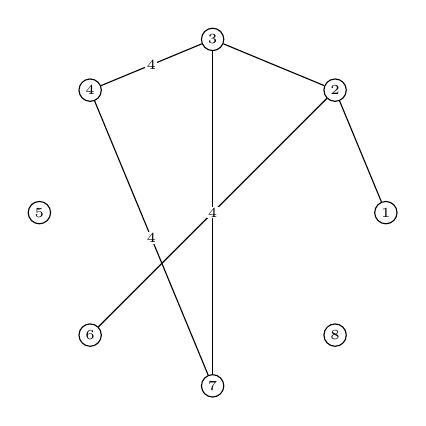
\begin{tikzpicture}[scale=2.2,v/.style={circle,draw,fill=white,inner sep=1.2pt,font=\tiny}]
  \node[v] (0) at (1.000,0.000) {1};
  \node[v] (1) at (0.707,0.707) {2};
  \node[v] (2) at (0.000,1.000) {3};
  \node[v] (3) at (-0.707,0.707) {4};
  \node[v] (4) at (-1.000,0.000) {5};
  \node[v] (5) at (-0.707,-0.707) {6};
  \node[v] (6) at (-0.000,-1.000) {7};
  \node[v] (7) at (0.707,-0.707) {8};
  \draw (0) -- (1);
  \draw (1) -- (2);
  \draw (1) -- node[fill=white,inner sep=0.5pt,font=\tiny] {8} (5);
  \draw (2) -- node[fill=white,inner sep=0.5pt,font=\tiny] {4} (3);
  \draw (2) -- node[fill=white,inner sep=0.5pt,font=\tiny] {4} (6);
  \draw (3) -- node[fill=white,inner sep=0.5pt,font=\tiny] {4} (6);
\end{tikzpicture}
}\\
$d=-1+3\sqrt2$, $n=2$ & $d=\sqrt2$, $n=4$\\[2mm]
\resizebox{0.36\textwidth}{!}{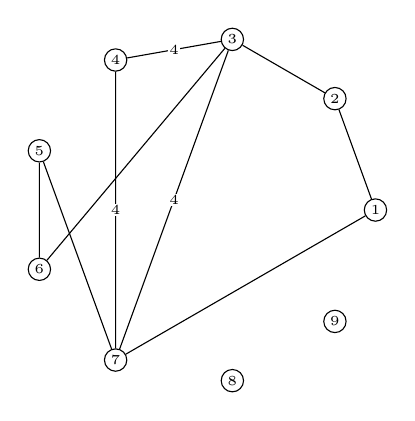
\begin{tikzpicture}[scale=2.2,v/.style={circle,draw,fill=white,inner sep=1.2pt,font=\tiny}]
  \node[v] (0) at (1.000,0.000) {1};
  \node[v] (1) at (0.766,0.643) {2};
  \node[v] (2) at (0.174,0.985) {3};
  \node[v] (3) at (-0.500,0.866) {4};
  \node[v] (4) at (-0.940,0.342) {5};
  \node[v] (5) at (-0.940,-0.342) {6};
  \node[v] (6) at (-0.500,-0.866) {7};
  \node[v] (7) at (0.174,-0.985) {8};
  \node[v] (8) at (0.766,-0.643) {9};
  \draw (0) -- (1);
  \draw (0) -- (6);
  \draw (1) -- (2);
  \draw (2) -- node[fill=white,inner sep=0.5pt,font=\tiny] {4} (3);
  \draw (2) -- (5);
  \draw (2) -- node[fill=white,inner sep=0.5pt,font=\tiny] {4} (6);
  \draw (3) -- node[fill=white,inner sep=0.5pt,font=\tiny] {4} (6);
  \draw (4) -- (5);
  \draw (4) -- (6);
\end{tikzpicture}
} &
\resizebox{0.36\textwidth}{!}{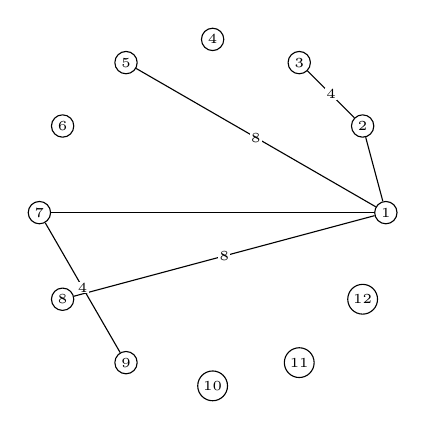
\begin{tikzpicture}[scale=2.2,v/.style={circle,draw,fill=white,inner sep=1.2pt,font=\tiny}]
  \node[v] (0) at (1.000,0.000) {1};
  \node[v] (1) at (0.866,0.500) {2};
  \node[v] (2) at (0.500,0.866) {3};
  \node[v] (3) at (0.000,1.000) {4};
  \node[v] (4) at (-0.500,0.866) {5};
  \node[v] (5) at (-0.866,0.500) {6};
  \node[v] (6) at (-1.000,0.000) {7};
  \node[v] (7) at (-0.866,-0.500) {8};
  \node[v] (8) at (-0.500,-0.866) {9};
  \node[v] (9) at (-0.000,-1.000) {10};
  \node[v] (10) at (0.500,-0.866) {11};
  \node[v] (11) at (0.866,-0.500) {12};
  \draw (0) -- (1);
  \draw (0) -- node[fill=white,inner sep=0.5pt,font=\tiny] {8} (4);
  \draw (0) -- (6);
  \draw (0) -- node[fill=white,inner sep=0.5pt,font=\tiny] {8} (7);
  \draw (1) -- node[fill=white,inner sep=0.5pt,font=\tiny] {4} (2);
  \draw (6) -- node[fill=white,inner sep=0.5pt,font=\tiny] {4} (8);
\end{tikzpicture}
}\\
$d=1+2\sqrt2$, $n=4$ & $d=3+3\sqrt2$, $n=3$\\[2mm]
\multicolumn{2}{c}{\resizebox{0.45\textwidth}{!}{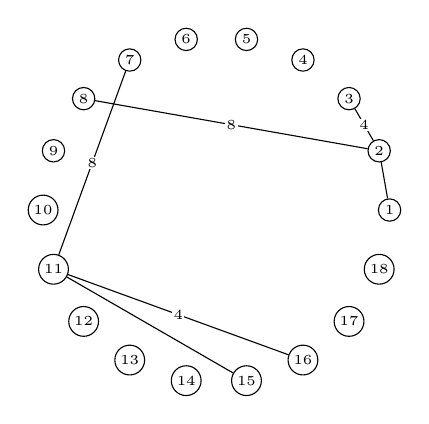
\begin{tikzpicture}[scale=2.2,v/.style={circle,draw,fill=white,inner sep=1.2pt,font=\tiny}]
  \node[v] (0) at (1.000,0.000) {1};
  \node[v] (1) at (0.940,0.342) {2};
  \node[v] (2) at (0.766,0.643) {3};
  \node[v] (3) at (0.500,0.866) {4};
  \node[v] (4) at (0.174,0.985) {5};
  \node[v] (5) at (-0.174,0.985) {6};
  \node[v] (6) at (-0.500,0.866) {7};
  \node[v] (7) at (-0.766,0.643) {8};
  \node[v] (8) at (-0.940,0.342) {9};
  \node[v] (9) at (-1.000,0.000) {10};
  \node[v] (10) at (-0.940,-0.342) {11};
  \node[v] (11) at (-0.766,-0.643) {12};
  \node[v] (12) at (-0.500,-0.866) {13};
  \node[v] (13) at (-0.174,-0.985) {14};
  \node[v] (14) at (0.174,-0.985) {15};
  \node[v] (15) at (0.500,-0.866) {16};
  \node[v] (16) at (0.766,-0.643) {17};
  \node[v] (17) at (0.940,-0.342) {18};
  \draw (0) -- (1);
  \draw (1) -- node[fill=white,inner sep=0.5pt,font=\tiny] {4} (2);
  \draw (1) -- node[fill=white,inner sep=0.5pt,font=\tiny] {8} (7);
  \draw (6) -- node[fill=white,inner sep=0.5pt,font=\tiny] {8} (10);
  \draw (10) -- (14);
  \draw (10) -- node[fill=white,inner sep=0.5pt,font=\tiny] {4} (15);
\end{tikzpicture}
}}\\
\multicolumn{2}{c}{$d=-2+3\sqrt2$, $n=3$}
\end{tabular}
\caption{Coxeter diagrams of new reflective cases. Vertices are facets. No edge means angle
$\pi/2$, an unlabelled edge $\pi/3$, and an edge labelled $k$ means $\pi/k$. Ultraparallel pairs (dotted edges) are omitted
for legibility. The full Gram matrices are in the ancillary files. The diagram for
$(\sqrt2,5)$, with 27 facets, is given only there.}\label{fig:new}
\end{figure}

\subsection{Observations}
\begin{itemize}
\item $\Nmax(d)$ falls quickly with $|\N(d)|$. Only the seven values with $|\N(d)|\le23$
  listed first in Table~\ref{tab:reflective} reach $n\ge3$, and none reaches $n\ge7$. This is
  far below the non-cocompact pattern over $\Q$, where $d=1,2,3$ reach $n=19,14,13$.
\item The two primes above a split $p$ can behave differently: $p=7$ ($\Nmax=5$ against $4$),
  $p=23$ ($3$ against $2$), $p=31$ ($\emptyset$ against $2$). Conjugate partners
  $d\leftrightarrow-\sigma(d)$ are not equivalent (\S\ref{sec:canonical}).
\item Among the \NCand{} candidates, \NNon{} minus one are non-reflective already at $n=2$:
  for them the table only contains non-diagonal lattices of determinant $(d)$.
\end{itemize}

\section{The gap in Mark's table and Hypothesis (D)}\label{sec:gap}

\subsection{Isometry testing by chamber matching}
\begin{proposition}\label{prop:matching}
Let $L_A,L_B$ be reflective rank-3 lattices with chambers $P_A,P_B$ and simple roots
$(a_i)$ and $(b_j)$. If $\varphi\colon L_A\to L_B$ is an isometry, then there is $w\in W(L_B)$
such that $w\varphi$ maps each $a_i$ to $u_i b_{\pi(i)}$ for an injection $\pi$ and units
$u_i>0$ at $\id$ with $u_i^2=(a_i,a_i)/(b_{\pi(i)},b_{\pi(i)})$.
\end{proposition}
\begin{proof}
$\varphi$ conjugates $W(L_A)$ onto $W(L_B)$, so $\varphi(P_A)$ is a chamber of $W(L_B)$ and
some $w\in W(L_B)$ maps it to $P_B$. Then $w\varphi$ maps facets to facets. A facet determines
its primitive outward root up to a positive unit.
\end{proof}
Hence, given the \emph{complete} simple-root cycle of $L_B$, enumerating the injections
compatible with the Gram matrices decides isometry. Any $\varphi$ obtained by solving on three
independent roots is accepted only if $\varphi$ and $\varphi^{-1}$ are integral and
$\varphi^TG_B\varphi=G_A$. For each reflective $d\in\mathcal C$ we tested
$\langle-d,1,1\rangle$ against every entry with determinant ideal $(d)$. Every one of them
except $d=-1+3\sqrt2$ is isometric to at least one entry (last column of
Table~\ref{tab:candidates}).

\subsection{The lattice $\langle1-3\sqrt2,1,1\rangle$}
Let $d=-1+3\sqrt2$, so $\N(d)=-17$ and $(d)$ is one of the primes above 17. Vinberg's algorithm
terminates with six roots. In cyclic order they are
\[
\begin{array}{lll}
e_1=(13+9\sqrt2,\,17+12\sqrt2,\,16+11\sqrt2), & (e_1,e_1)=2+\sqrt2,\\
e_2=(0,-1,1), & (e_2,e_2)=2,\\
e_3=(0,0,-1), & (e_3,e_3)=1,\\
e_4=(3+2\sqrt2,\,5+4\sqrt2,\,0), & (e_4,e_4)=2+\sqrt2,\\
e_5=(2+\sqrt2,\,3+2\sqrt2,\,1+\sqrt2), & (e_5,e_5)=2,\\
e_6=(4+3\sqrt2,\,6+4\sqrt2,\,5+3\sqrt2), & (e_6,e_6)=1,
\end{array}
\]
with consecutive inner products
$(e_1,e_2)=(e_4,e_5)=-1-\sqrt2$, $(e_2,e_3)=(e_5,e_6)=-1$ and $(e_3,e_4)=(e_6,e_1)=0$. The
chamber is therefore a compact hexagon with angles
$(\pi/8,\pi/4,\pi/2,\pi/8,\pi/4,\pi/2)$; CoxIter gives $\chi=-9/8$. The independent rank-3
implementation of \S\ref{sec:vinberg3} was started from an interior point of this hexagon. It
also terminates with exactly these six roots.

Mark's table has 8 entries with determinant ideal $(-1+3\sqrt2)$. Their shapes are $(322)^2$
(two entries) and $(2222)^2$ (six entries); none has angle cycle $842842$. The angle cycle of
the chamber is an isometry invariant, so none of these entries is isometric to
$\langle-d,1,1\rangle$. This argument relies on the printed shapes. To remove that dependence, we recomputed the
full chambers of all 8 entries with the implementation of \S\ref{sec:vinberg3}. Each run
terminates and contains the printed roots. The two $(322)^2$ entries are hexagons with
angles $(\pi/3,\pi/2,\pi/2)^2$, and the six $(2222)^2$ entries are octagons. So none of them
is an $842842$ hexagon, independently of the printed data. The only hexagon of shape $(842)^2$ in the whole table has
determinant ideal $(1+3\sqrt2)$, the other prime above 17. That entry is explicitly isometric
to $\langle-(1+3\sqrt2),1,1\rangle$, and the two hexagons have identical angles and root
norms.

\begin{proposition}\label{prop:gap}
$\langle1-3\sqrt2,1,1\rangle$ is a reflective strongly squarefree rank-3 lattice over $\OK$
that is isometric to no entry of the table in~\cite{Mar18}.
\end{proposition}

We do not know the cause. One possibility is that the enumeration identified the two
hexagons over the conjugate primes above 17, which have identical combinatorics and norms.
Another is an omission at some stage of the enumeration or of typesetting. The published
version of~\cite{Mar18} has not been compared with the arXiv source.

\subsection{What completeness rests on}
Proposition~\ref{prop:gap} shows that Theorem~\ref{thm:mark} cannot be used as stated.
Corollary~\ref{cor:reduction} only needs the weaker statement:

\begin{hypothesis}
For every reflective strongly squarefree rank-3 lattice $L$ over $\Z[\sqrt2]$, the ideal
$(\det L)$ is the determinant ideal of some entry of Mark's table, i.e.\ belongs to the
$\NCand$ ideals of Appendix~\ref{app:candidates}.
\end{hypothesis}

Proposition~\ref{prop:gap} does not contradict (D), because $(-1+3\sqrt2)$ does occur in the
table. But it shows that the table can miss a reflective lattice whose determinant ideal is
otherwise represented. Nothing excludes an omission whose ideal is not represented. Two partial
safeguards:
\begin{enumerate}
\item \emph{Conjugate partners.} If the gap arose from identifying conjugate primes, its most
  likely trace is a reflective $d$ whose partner $-\sigma(d)$ is not a candidate. We
  computed $-\sigma(d)$ for each of the \NRefl{} reflective $d$. All are candidates except
  $5+6\sqrt2$ (partner of $-5+6\sqrt2$), which is certified non-reflective at $n=2$ in the
  grid, and $-1+12\sqrt2$ (partner of $1+12\sqrt2$). We decided $-1+12\sqrt2$ directly: it is
  non-reflective at $n=2$, with a certificate. Partners are not equivalent in general: for
  example, $1+4\sqrt2$ is reflective and $-1+4\sqrt2$ is not. So this check shows only that
  no partner-type omission occurs among our reflective $d$.
\item \emph{Independent grid.} For all 16 prime or unit parameters with
  $|\N(\mathfrak p)|\le50$ our own computation agrees with membership in~$\mathcal C$
  (\S\ref{sec:extract}).
\end{enumerate}
Proving (D) unconditionally would need an independent rank-3 classification, or a
re-verification of the relevant part of~\cite{Mar18}, for example of the Allcock--Nikulin
type bounds on short and close pairs of roots. We have not attempted this.

\section{Comparison with the literature}\label{sec:literature}
Every reflective pair $(d,n)$ was compared with the following sources, after checking
isometry explicitly.
\begin{itemize}
\item \emph{$n=2$.} An explicit isometry to a table entry of~\cite{Mar18}; this covers every
  case except $d=-1+3\sqrt2$.
\item \emph{$d=\eps$.} Reflective iff $n\le6$~\cite{Bug90}, as cited
  in~\cite{Gug17,Bel16}; we did not have access to~\cite{Bug90} itself.
\item \emph{$n=3$.} Bogachev's list of candidate lattices $L(1)$--$L(11)$ in~\cite{Bog20}:
  \begin{itemize}
  \item the diagonal rows $L(1),L(2),L(3),L(5)$ are $d=\eps$, $1+2\sqrt2$, $-1+2\sqrt2$
    (as $5+4\sqrt2=(-1+2\sqrt2)\eps^2$) and $\sqrt2$;
  \item $L(8)=\langle-(7+6\sqrt2),1,1,1\rangle$ is $d=-3+4\sqrt2$, since
    $7+6\sqrt2=(-3+4\sqrt2)\eps^2$. Bogachev shows it is reflective but not
    sub-$2$-reflective;
  \item his non-diagonal rows $L(6),L(7),L(10),L(11)$ have determinant ideals $(2+3\sqrt2)$,
    $(2+3\sqrt2)$, $(3+4\sqrt2)$ and $(11+12\sqrt2)$. So they cover neither $3+3\sqrt2$ nor
    $-2+3\sqrt2$.
  \end{itemize}
\item \emph{$d=-1+2\sqrt2$.} Reflective for $n\le5$ by Guglielmetti~\cite{Gug17}, via
  $\langle1-2\Theta_2,1,1,1,1\rangle$ and $\langle-5-4\Theta_2,1,\dots,1\rangle$ with
  $\Theta_2=\sqrt2$. Our $n=5$ polytope has 20 facets and $f$-vector
  $(96,240,228,102,20,1)$, as in~\cite{Gug17}.
\end{itemize}
The remaining reflective pairs are, as far as these sources go, new:
\[
 (-1+3\sqrt2,2),\quad(\sqrt2,4),\quad(\sqrt2,5),\quad(1+2\sqrt2,4),\quad(3+3\sqrt2,3),\quad(-2+3\sqrt2,3).
\]
The upper ends $\Nmax(d)$ were known before only for $\eps$~\cite{Bug90} and, in effect, for
$-1+2\sqrt2$~\cite{Gug17}. For the candidates that are non-reflective at $n=2$,
non-reflectivity at $n=2$ also follows from~\cite{Mar18}.

\begin{remark}[Non-reduced coefficients]\label{rem:alvin}
Bogachev's rows $L(4)=\langle-(11+8\sqrt2),1,1,1\rangle$ and $L(9)=\langle-(7+5\sqrt2),1,1,1\rangle$
are isometric to $L(2)$ and $L(1)$, since $11+8\sqrt2=(1+2\sqrt2)\eps^2$ and
$7+5\sqrt2=\eps^3$. Their printed root lists nevertheless differ from those of $L(2)$ and
$L(1)$. AlVin reproduces the printed lists. In both cases the root $(\sqrt2-1,1+\sqrt2,0,0)$
should be accepted first and is missed. The likely cause is that candidates with
$0<k_0<1$ at $\id$ are skipped, which matters only when the coefficient is not reduced modulo
unit squares. Our implementation gives the same chamber for $d$ and $d\eps^{2k}$; this is
tested. Bogachev's conclusions about $L(4)$ and $L(9)$ are unaffected, because those lattices
are isometric to $L(2)$ and $L(1)$.
\end{remark}

\section{Calibration and cross-checks}\label{sec:calibration}
The same code, with the ring interface instantiated to $\Z$, reproduces the following.
\begin{itemize}
\item \emph{Over $\Q$:} $p=3$ reflective iff $n\le13$~\cite{Mc11}; $p=5$ iff
  $n\le8$~\cite{Mar15}; and the maxima $3,4,2,3,2,2$ for $d=7,11,13,17,19,23$ of
  \cite[Table~3.1]{McTh}.
\item \emph{$d=\eps$:} terminates for $n\le6$ and not at $n=7$~\cite{Bug90}. Our certificate
  at $n=7$ makes the latter rigorous.
\item \emph{$d=-1+2\sqrt2$:} the facet count and $f$-vector of Guglielmetti's $n=5$
  polytope~\cite{Gug17}.
\item \emph{AlVin:} identical root sets for nine pairs $(d,n)$ over $\Z$ and $\OK$.
\item \emph{CoxIter:} compactness, $f$-vector and Euler characteristic of every reflective
  case.
\end{itemize}
In addition:
\begin{itemize}
\item \emph{Facet test} (from Lemma~\ref{lem:mono}): for all 14 grid pairs where both
  $(d,n)$ and $(d,n+1)$ are reflective, the facet $v_{n+1}^\perp$ of the $(d,n+1)$ chamber
  reproduces the $(d,n)$ chamber exactly.
\item \emph{Rescaling:} $d$ and $d\eps^{2k}$ give the same chamber
  (Remark~\ref{rem:alvin}).
\item \emph{The table:} the seven exact checks of \S\ref{sec:extract} on all \NEntries{}
  entries.
\end{itemize}
Finally, for each certified case of the grid we searched for a reflective super-lattice
$L'\supset L$ in which the infinite-order symmetry becomes a product of reflections (cf.\
\cite[Fig.~3.2]{McTh}). None was found within the caps used. This is recorded as ``not found'',
not as a negative result.

\section{Reproducibility}\label{sec:repro}
The software is written in Python, with exact arithmetic in \texttt{fractions.Fraction}. It
is available at \texttt{[URL to be added]}. The ancillary files of this submission contain:
\begin{itemize}
\item the verifier \texttt{verify\_certificate.py} together with the package \texttt{reflect/};
\item all \NCerts{} certificates;
\item for every reflective case, the roots, Gram matrix and Coxeter diagram;
\item the per-$d$ summary \texttt{classification.json};
\item the stored isometries to table entries;
\item the parser for Mark's \TeX{} source. The table itself is not redistributed and is
  regenerated from arXiv:1512.01133.
\end{itemize}
The test suite (913 tests) re-verifies every certificate and stored isometry, the table
checks, the calibrations and the literature attributions. One uncertain step is isolated in
\S\ref{sec:certificates}: elliptic subdiagrams correspond to vertices for chambers with
infinitely many facets.

\subsection*{Acknowledgements}
% TODO(author): review this disclosure and adapt it to arXiv's policy on AI tools.
The software, the computations and a first draft of this report were produced with the
assistance of Claude (Anthropic), an AI system, under the author's direction. The author has
reviewed the mathematics and is responsible for the content. We thank the authors of AlVin
and CoxIter for making their software available.

\begin{thebibliography}{99}
% TODO(author): check every reference against the published versions.
\bibitem{All12} D.~Allcock, \emph{The reflective Lorentzian lattices of rank 3},
  Mem. Amer. Math. Soc. \textbf{220} (2012), no.~1033.
\bibitem{Bel16} M.~Belolipetsky, \emph{Arithmetic hyperbolic reflection groups},
  Bull. Amer. Math. Soc. \textbf{53} (2016), 437--475; arXiv:1506.03111.
\bibitem{Bog20} N.~Bogachev, \emph{From geometry to arithmetic of compact hyperbolic Coxeter
  polytopes}, arXiv:2003.11944.
\bibitem{Bug90} V.~O.~Bugaenko, % TODO(author): full title and pages
  Selecta Math. Soviet. \textbf{9} (1990).
\bibitem{CoxIter} R.~Guglielmetti, \emph{CoxIter -- computing invariants of hyperbolic Coxeter
  groups}, LMS J. Comput. Math. \textbf{18} (2015), 754--773.
\bibitem{AlVin} R.~Guglielmetti, \emph{AlVin: a C++ implementation of the Vinberg algorithm
  for diagonal quadratic forms}, \url{https://github.com/rgugliel/AlVin}.
\bibitem{Gug17} R.~Guglielmetti, \emph{Hyperbolic isometries in (in-)finite dimensions and
  discrete reflection groups: theory and computations}, PhD thesis, Universit\'e de
  Fribourg, 2017. % TODO(author): confirm title
\bibitem{Mar15} A.~Mark, \emph{Reflection groups of the quadratic form
  $-px_0^2+x_1^2+\dots+x_n^2$ with $p$ prime}, Publ. Mat. \textbf{59} (2015), 353--372;
  arXiv:1207.4822.
\bibitem{Mar18} A.~Mark, \emph{The classification of rank 3 reflective hyperbolic lattices
  over $\Z[\sqrt2]$}, Math. Proc. Cambridge Philos. Soc. \textbf{164} (2018), 221--257;
  arXiv:1512.01133.
\bibitem{Mc11} J.~Mcleod, \emph{Hyperbolic reflection groups associated to the quadratic
  forms $-3x_0^2+x_1^2+\dots+x_n^2$}, arXiv:1007.2299. % TODO(author): journal reference
\bibitem{McTh} J.~Mcleod, \emph{Arithmetic hyperbolic reflection groups}, PhD thesis,
  Durham University, 2013. % TODO(author): confirm title
\bibitem{Nik00} V.~V.~Nikulin, \emph{On the classification of hyperbolic root systems of
  rank three}, arXiv:alg-geom/9711032.
\bibitem{Vin72} E.~B.~Vinberg, \emph{On groups of unit elements of certain quadratic forms},
  Math. USSR Sb. \textbf{16} (1972), 17--35.
\bibitem{Vin85} E.~B.~Vinberg, \emph{The absence of crystallographic groups of reflections in
  Lobachevsky spaces of large dimension}, Trans. Moscow Math. Soc. (1985), 75--112.
\end{thebibliography}

\appendix
\section{All candidates}\label{app:candidates}

{\footnotesize
\begin{longtable}{llrlrll}
\caption{The \NCand{} candidates $d=\mathrm{can}((\delta_e))$ from Mark's table, and
$-1+12\sqrt2$ ($\dagger$, conjugate partner of $1+12\sqrt2$, not a candidate). Columns: label,
$d$, $\N(d)$, factorisation, number of table entries with determinant ideal $(d)$, result at
$n=2$ (R: reflective, with number of facets; N: non-reflective, with the number of roots found
before the certificate search), and for reflective $d$ the number of those entries isometric to
$\langle-d,1,1\rangle$.}\label{tab:candidates}\\
\toprule
label & $d$ & $\N(d)$ & $(d)$ & entries & $n=2$ & isometric\\
\midrule\endfirsthead
\toprule
label & $d$ & $\N(d)$ & $(d)$ & entries & $n=2$ & isometric\\
\midrule\endhead
\texttt{unit} & $1+\sqrt2$ & $-1$ & $\text{unit}$ & 1 & R (3) & 1/1 \\
\texttt{ram2} & $\sqrt2$ & $-2$ & $(\sqrt2)$ & 2 & R (4) & 1/2 \\
\texttt{p7a} & $-1+2\sqrt2$ & $-7$ & $(3+\sqrt2)$ & 10 & R (4) & 6/10 \\
\texttt{p7b} & $1+2\sqrt2$ & $-7$ & $(3-\sqrt2)$ & 13 & R (4) & 1/13 \\
\texttt{inert3} & $3+3\sqrt2$ & $-9$ & $(3)$ & 5 & R (4) & 2/5 \\
\texttt{d2\_3} & $2+3\sqrt2$ & $-14$ & $(\sqrt2)\cdot(3+\sqrt2)$ & 13 & R (5) & 2/13 \\
\texttt{dm2\_3} & $-2+3\sqrt2$ & $-14$ & $(\sqrt2)\cdot(3-\sqrt2)$ & 15 & R (5) & 3/15 \\
\texttt{p17a} & $-1+3\sqrt2$ & $-17$ & $(5+2\sqrt2)$ & 8 & R (6) & 0/8 \\
\texttt{p17b} & $1+3\sqrt2$ & $-17$ & $(5-2\sqrt2)$ & 8 & R (6) & 1/8 \\
\texttt{d0\_3} & $3\sqrt2$ & $-18$ & $(\sqrt2)\cdot(3)$ & 6 & R (6) & 3/6 \\
\texttt{p23a} & $-3+4\sqrt2$ & $-23$ & $(5+\sqrt2)$ & 6 & R (5) & 3/6 \\
\texttt{p23b} & $3+4\sqrt2$ & $-23$ & $(5-\sqrt2)$ & 8 & R (6) & 1/8 \\
\texttt{inert5} & $5+5\sqrt2$ & $-25$ & $(5)$ & 5 & R (6) & 5/5 \\
\texttt{p31a} & $-1+4\sqrt2$ & $-31$ & $(7+3\sqrt2)$ & 5 & N (9 roots) & -- \\
\texttt{p31b} & $1+4\sqrt2$ & $-31$ & $(7-3\sqrt2)$ & 5 & R (8) & 2/5 \\
\texttt{d4\_5} & $4+5\sqrt2$ & $-34$ & $(\sqrt2)\cdot(5+2\sqrt2)$ & 12 & N (34 roots) & -- \\
\texttt{dm4\_5} & $-4+5\sqrt2$ & $-34$ & $(\sqrt2)\cdot(5-2\sqrt2)$ & 10 & N (22 roots) & -- \\
\texttt{p41a} & $-3+5\sqrt2$ & $-41$ & $(7+2\sqrt2)$ & 2 & R (12) & 2/2 \\
\texttt{p41b} & $3+5\sqrt2$ & $-41$ & $(7-2\sqrt2)$ & 2 & R (12) & 2/2 \\
\texttt{d2\_5} & $2+5\sqrt2$ & $-46$ & $(\sqrt2)\cdot(5+\sqrt2)$ & 8 & N (43 roots) & -- \\
\texttt{dm2\_5} & $-2+5\sqrt2$ & $-46$ & $(\sqrt2)\cdot(5-\sqrt2)$ & 6 & N (45 roots) & -- \\
\texttt{p47a} & $-5+6\sqrt2$ & $-47$ & $(7+\sqrt2)$ & 6 & R (10) & 4/6 \\
\texttt{d7\_7} & $7+7\sqrt2$ & $-49$ & $(3+\sqrt2)\cdot(3-\sqrt2)$ & 23 & R (5) & 2/23 \\
\texttt{d0\_5} & $5\sqrt2$ & $-50$ & $(\sqrt2)\cdot(5)$ & 2 & N (44 roots) & -- \\
\texttt{d6\_7} & $6+7\sqrt2$ & $-62$ & $(\sqrt2)\cdot(7+3\sqrt2)$ & 8 & N (101 roots) & -- \\
\texttt{dm6\_7} & $-6+7\sqrt2$ & $-62$ & $(\sqrt2)\cdot(7-3\sqrt2)$ & 4 & R (11) & 3/4 \\
\texttt{d3\_6} & $3+6\sqrt2$ & $-63$ & $(3)\cdot(3-\sqrt2)$ & 24 & R (8) & 2/24 \\
\texttt{dm3\_6} & $-3+6\sqrt2$ & $-63$ & $(3)\cdot(3+\sqrt2)$ & 23 & N (21 roots) & -- \\
\texttt{d4\_7} & $4+7\sqrt2$ & $-82$ & $(\sqrt2)\cdot(7+2\sqrt2)$ & 3 & N (94 roots) & -- \\
\texttt{dm4\_7} & $-4+7\sqrt2$ & $-82$ & $(\sqrt2)\cdot(7-2\sqrt2)$ & 3 & N (48 roots) & -- \\
\texttt{d2\_7} & $2+7\sqrt2$ & $-94$ & $(\sqrt2)\cdot(7+\sqrt2)$ & 1 & N (41 roots) & -- \\
\texttt{dm2\_7} & $-2+7\sqrt2$ & $-94$ & $(\sqrt2)\cdot(7-\sqrt2)$ & 4 & N (57 roots) & -- \\
\texttt{d0\_7} & $7\sqrt2$ & $-98$ & $(\sqrt2)\cdot(3+\sqrt2)\cdot(3-\sqrt2)$ & 23 & R (8) & 2/23 \\
\texttt{d3\_8} & $3+8\sqrt2$ & $-119$ & $(3+\sqrt2)\cdot(5+2\sqrt2)$ & 6 & N (70 roots) & -- \\
\texttt{d9\_10} & $9+10\sqrt2$ & $-119$ & $(3+\sqrt2)\cdot(5-2\sqrt2)$ & 10 & R (8) & 3/10 \\
\texttt{dm3\_8} & $-3+8\sqrt2$ & $-119$ & $(3-\sqrt2)\cdot(5-2\sqrt2)$ & 8 & N (15 roots) & -- \\
\texttt{dm9\_10} & $-9+10\sqrt2$ & $-119$ & $(3-\sqrt2)\cdot(5+2\sqrt2)$ & 6 & R (12) & 3/6 \\
\texttt{d6\_9} & $6+9\sqrt2$ & $-126$ & $(\sqrt2)\cdot(3)\cdot(3+\sqrt2)$ & 30 & N (35 roots) & -- \\
\texttt{dm6\_9} & $-6+9\sqrt2$ & $-126$ & $(\sqrt2)\cdot(3)\cdot(3-\sqrt2)$ & 27 & R (11) & 5/27 \\
\texttt{d4\_9} & $4+9\sqrt2$ & $-146$ & $(\sqrt2)\cdot(9+2\sqrt2)$ & 2 & N (154 roots) & -- \\
\texttt{dm4\_9} & $-4+9\sqrt2$ & $-146$ & $(\sqrt2)\cdot(9-2\sqrt2)$ & 3 & N (106 roots) & -- \\
\texttt{dm2\_9} & $-2+9\sqrt2$ & $-158$ & $(\sqrt2)\cdot(9-\sqrt2)$ & 5 & N (117 roots) & -- \\
\texttt{d1\_9} & $1+9\sqrt2$ & $-161$ & $(3-\sqrt2)\cdot(5-\sqrt2)$ & 4 & R (18) & 4/4 \\
\texttt{d9\_11} & $9+11\sqrt2$ & $-161$ & $(3-\sqrt2)\cdot(5+\sqrt2)$ & 3 & N (52 roots) & -- \\
\texttt{dm1\_9} & $-1+9\sqrt2$ & $-161$ & $(3+\sqrt2)\cdot(5+\sqrt2)$ & 6 & R (18) & 3/6 \\
\texttt{dm9\_11} & $-9+11\sqrt2$ & $-161$ & $(3+\sqrt2)\cdot(5-\sqrt2)$ & 7 & N (50 roots) & -- \\
\texttt{d4\_11} & $4+11\sqrt2$ & $-226$ & $(\sqrt2)\cdot(11+2\sqrt2)$ & 2 & N (84 roots) & -- \\
\texttt{dm4\_11} & $-4+11\sqrt2$ & $-226$ & $(\sqrt2)\cdot(11-2\sqrt2)$ & 2 & N (136 roots) & -- \\
\texttt{d10\_13} & $10+13\sqrt2$ & $-238$ & $(\sqrt2)\cdot(3-\sqrt2)\cdot(5-2\sqrt2)$ & 9 & N (83 roots) & -- \\
\texttt{d2\_11} & $2+11\sqrt2$ & $-238$ & $(\sqrt2)\cdot(3-\sqrt2)\cdot(5+2\sqrt2)$ & 10 & N (104 roots) & -- \\
\texttt{dm10\_13} & $-10+13\sqrt2$ & $-238$ & $(\sqrt2)\cdot(3+\sqrt2)\cdot(5+2\sqrt2)$ & 10 & N (165 roots) & -- \\
\texttt{dm2\_11} & $-2+11\sqrt2$ & $-238$ & $(\sqrt2)\cdot(3+\sqrt2)\cdot(5-2\sqrt2)$ & 7 & N (129 roots) & -- \\
\texttt{d1\_12} & $1+12\sqrt2$ & $-287$ & $(3+\sqrt2)\cdot(7+2\sqrt2)$ & 5 & R (24) & 5/5 \\
\texttt{dm1\_12}$^\dagger$ & $-1+12\sqrt2$ & $-287$ & $(3-\sqrt2)\cdot(7-2\sqrt2)$ & 0 & N (125 roots) & -- \\
\texttt{d12\_15} & $12+15\sqrt2$ & $-306$ & $(\sqrt2)\cdot(3)\cdot(5+2\sqrt2)$ & 3 & N (122 roots) & -- \\
\texttt{dm12\_15} & $-12+15\sqrt2$ & $-306$ & $(\sqrt2)\cdot(3)\cdot(5-2\sqrt2)$ & 5 & N (62 roots) & -- \\
\texttt{d16\_17} & $16+17\sqrt2$ & $-322$ & $(\sqrt2)\cdot(3+\sqrt2)\cdot(5+\sqrt2)$ & 13 & N (108 roots) & -- \\
\texttt{d4\_13} & $4+13\sqrt2$ & $-322$ & $(\sqrt2)\cdot(3+\sqrt2)\cdot(5-\sqrt2)$ & 2 & N (101 roots) & -- \\
\texttt{dm16\_17} & $-16+17\sqrt2$ & $-322$ & $(\sqrt2)\cdot(3-\sqrt2)\cdot(5-\sqrt2)$ & 13 & N (94 roots) & -- \\
\texttt{dm4\_13} & $-4+13\sqrt2$ & $-322$ & $(\sqrt2)\cdot(3-\sqrt2)\cdot(5+\sqrt2)$ & 2 & N (103 roots) & -- \\
\texttt{dm10\_15} & $-10+15\sqrt2$ & $-350$ & $(\sqrt2)\cdot(5)\cdot(3-\sqrt2)$ & 8 & N (177 roots) & -- \\
\texttt{d6\_15} & $6+15\sqrt2$ & $-414$ & $(\sqrt2)\cdot(3)\cdot(5+\sqrt2)$ & 5 & N (161 roots) & -- \\
\texttt{d12\_17} & $12+17\sqrt2$ & $-434$ & $(\sqrt2)\cdot(3-\sqrt2)\cdot(7-3\sqrt2)$ & 2 & N (158 roots) & -- \\
\texttt{d4\_15} & $4+15\sqrt2$ & $-434$ & $(\sqrt2)\cdot(3-\sqrt2)\cdot(7+3\sqrt2)$ & 3 & N (99 roots) & -- \\
\texttt{dm12\_17} & $-12+17\sqrt2$ & $-434$ & $(\sqrt2)\cdot(3+\sqrt2)\cdot(7+3\sqrt2)$ & 3 & N (154 roots) & -- \\
\texttt{dm4\_15} & $-4+15\sqrt2$ & $-434$ & $(\sqrt2)\cdot(3+\sqrt2)\cdot(7-3\sqrt2)$ & 4 & N (180 roots) & -- \\
\texttt{d21\_21} & $21+21\sqrt2$ & $-441$ & $(3)\cdot(3+\sqrt2)\cdot(3-\sqrt2)$ & 4 & N (133 roots) & -- \\
\texttt{d6\_21} & $6+21\sqrt2$ & $-846$ & $(\sqrt2)\cdot(3)\cdot(7+\sqrt2)$ & 3 & N (125 roots) & -- \\
\texttt{d0\_21} & $21\sqrt2$ & $-882$ & $(\sqrt2)\cdot(3)\cdot(3+\sqrt2)\cdot(3-\sqrt2)$ & 10 & N (158 roots) & -- \\
\texttt{d28\_35} & $28+35\sqrt2$ & $-1666$ & $(\sqrt2)\cdot(3+\sqrt2)\cdot(3-\sqrt2)\cdot(5+2\sqrt2)$ & 3 & N (180 roots) & -- \\
\texttt{dm28\_35} & $-28+35\sqrt2$ & $-1666$ & $(\sqrt2)\cdot(3+\sqrt2)\cdot(3-\sqrt2)\cdot(5-2\sqrt2)$ & 3 & N (234 roots) & -- \\
\bottomrule

\end{longtable}}

{\footnotesize
\begin{longtable}{lrrrl}
\caption{The certificate at $n_0=\Nmax(d)+1$ for each $d$: number of Vinberg roots used,
number of vertex symmetries in the product $g$, and a rational interval containing a real
eigenvalue $>1$ of $g$.}\label{tab:certs}\\
\toprule
label & $n_0$ & roots & factors & eigenvalue in\\
\midrule\endfirsthead
\toprule
label & $n_0$ & roots & factors & eigenvalue in\\
\midrule\endhead
\texttt{unit} & 7 & 80 & 2 & $[39/2, 20]$ \\
\texttt{ram2} & 6 & 40 & 1 & $[21/2, 11]$ \\
\texttt{p7a} & 6 & 80 & 1 & $[5/2, 3]$ \\
\texttt{p7b} & 5 & 33 & 1 & $[19/2, 10]$ \\
\texttt{inert3} & 4 & 40 & 1 & $[6, 13/2]$ \\
\texttt{d2\_3} & 3 & 20 & 2 & $[12, 25/2]$ \\
\texttt{dm2\_3} & 4 & 40 & 2 & $[13/2, 7]$ \\
\texttt{p17a} & 3 & 20 & 2 & $[19/2, 10]$ \\
\texttt{p17b} & 3 & 20 & 2 & $[75/2, 38]$ \\
\texttt{d0\_3} & 3 & 33 & 2 & $[113/2, 57]$ \\
\texttt{p23a} & 4 & 20 & 2 & $[27/2, 14]$ \\
\texttt{p23b} & 3 & 20 & 1 & $[27, 55/2]$ \\
\texttt{inert5} & 3 & 31 & 2 & $[37/2, 19]$ \\
\texttt{p31a} & 2 & 9 & 2 & $[607/2, 304]$ \\
\texttt{p31b} & 3 & 18 & 2 & $[212, 425/2]$ \\
\texttt{d4\_5} & 2 & 20 & 2 & $[19/2, 10]$ \\
\texttt{dm4\_5} & 2 & 20 & 1 & $[205/2, 103]$ \\
\texttt{p41a} & 3 & 40 & 2 & $[177/2, 89]$ \\
\texttt{p41b} & 3 & 40 & 2 & $[131/2, 66]$ \\
\texttt{d2\_5} & 2 & 20 & 1 & $[19/2, 10]$ \\
\texttt{dm2\_5} & 2 & 20 & 1 & $[19/2, 10]$ \\
\texttt{p47a} & 3 & 20 & 2 & $[10, 21/2]$ \\
\texttt{d7\_7} & 3 & 80 & 1 & $[11/2, 6]$ \\
\texttt{d0\_5} & 2 & 40 & 1 & $[21, 43/2]$ \\
\texttt{d6\_7} & 2 & 20 & 2 & $[89/2, 45]$ \\
\texttt{dm6\_7} & 3 & 157 & 1 & $[81/2, 41]$ \\
\texttt{d3\_6} & 3 & 37 & 2 & $[1643/2, 822]$ \\
\texttt{dm3\_6} & 2 & 20 & 1 & $[15, 31/2]$ \\
\texttt{d4\_7} & 2 & 40 & 1 & $[21, 43/2]$ \\
\texttt{dm4\_7} & 2 & 48 & 1 & $[131/2, 66]$ \\
\texttt{d2\_7} & 2 & 40 & 2 & $[205/2, 103]$ \\
\texttt{dm2\_7} & 2 & 20 & 2 & $[205/2, 103]$ \\
\texttt{d0\_7} & 3 & 142 & 1 & $[117/2, 59]$ \\
\texttt{d3\_8} & 2 & 20 & 1 & $[11/2, 6]$ \\
\texttt{d9\_10} & 3 & 40 & 2 & $[21, 43/2]$ \\
\texttt{dm3\_8} & 2 & 15 & 2 & $[3054, 6109/2]$ \\
\texttt{dm9\_10} & 3 & 40 & 2 & $[225/2, 113]$ \\
\texttt{d6\_9} & 2 & 20 & 2 & $[205/2, 103]$ \\
\texttt{dm6\_9} & 3 & 160 & 2 & $[39/2, 20]$ \\
\texttt{d4\_9} & 2 & 40 & 1 & $[19/2, 10]$ \\
\texttt{dm4\_9} & 2 & 20 & 2 & $[267/2, 134]$ \\
\texttt{dm2\_9} & 2 & 20 & 2 & $[5293, 10587/2]$ \\
\texttt{d1\_9} & 3 & 157 & 2 & $[16, 33/2]$ \\
\texttt{d9\_11} & 2 & 40 & 1 & $[39/2, 20]$ \\
\texttt{dm1\_9} & 3 & 191 & 1 & $[23/2, 12]$ \\
\texttt{dm9\_11} & 2 & 40 & 1 & $[25/2, 13]$ \\
\texttt{d4\_11} & 2 & 80 & 2 & $[11603/2, 5802]$ \\
\texttt{dm4\_11} & 2 & 40 & 2 & $[267/2, 134]$ \\
\texttt{d10\_13} & 2 & 40 & 2 & $[89/2, 45]$ \\
\texttt{d2\_11} & 2 & 40 & 1 & $[61, 123/2]$ \\
\texttt{dm10\_13} & 2 & 40 & 2 & $[1813/2, 907]$ \\
\texttt{dm2\_11} & 2 & 40 & 1 & $[23, 47/2]$ \\
\texttt{d1\_12} & 3 & 160 & 1 & $[49/2, 25]$ \\
\texttt{dm1\_12} & 2 & 40 & 1 & $[7, 15/2]$ \\
\texttt{d12\_15} & 2 & 40 & 1 & $[135/2, 68]$ \\
\texttt{dm12\_15} & 2 & 62 & 2 & $[205/2, 103]$ \\
\texttt{d16\_17} & 2 & 80 & 1 & $[21, 43/2]$ \\
\texttt{d4\_13} & 2 & 80 & 1 & $[126, 253/2]$ \\
\texttt{dm16\_17} & 2 & 80 & 1 & $[337/2, 169]$ \\
\texttt{dm4\_13} & 2 & 80 & 1 & $[679/2, 340]$ \\
\texttt{dm10\_15} & 2 & 40 & 1 & $[61, 123/2]$ \\
\texttt{d6\_15} & 2 & 20 & 2 & $[712, 1425/2]$ \\
\texttt{d12\_17} & 2 & 40 & 2 & $[2502, 5005/2]$ \\
\texttt{d4\_15} & 2 & 80 & 2 & $[51589, 103179/2]$ \\
\texttt{dm12\_17} & 2 & 40 & 2 & $[3395, 6791/2]$ \\
\texttt{dm4\_15} & 2 & 20 & 1 & $[23, 47/2]$ \\
\texttt{d21\_21} & 2 & 40 & 1 & $[69/2, 35]$ \\
\texttt{d6\_21} & 2 & 80 & 1 & $[712, 1425/2]$ \\
\texttt{d0\_21} & 2 & 80 & 1 & $[93/2, 47]$ \\
\texttt{d28\_35} & 2 & 160 & 1 & $[595/2, 298]$ \\
\texttt{dm28\_35} & 2 & 80 & 1 & $[262, 525/2]$ \\
\bottomrule

\end{longtable}}

\end{document}
